% Options for packages loaded elsewhere
\PassOptionsToPackage{unicode}{hyperref}
\PassOptionsToPackage{hyphens}{url}
%
\documentclass[
  12pt,
  landscape]{article}
\usepackage{lmodern}
\usepackage{amssymb,amsmath}
\usepackage{ifxetex,ifluatex}
\ifnum 0\ifxetex 1\fi\ifluatex 1\fi=0 % if pdftex
  \usepackage[T1]{fontenc}
  \usepackage[utf8]{inputenc}
  \usepackage{textcomp} % provide euro and other symbols
\else % if luatex or xetex
  \usepackage{unicode-math}
  \defaultfontfeatures{Scale=MatchLowercase}
  \defaultfontfeatures[\rmfamily]{Ligatures=TeX,Scale=1}
\fi
% Use upquote if available, for straight quotes in verbatim environments
\IfFileExists{upquote.sty}{\usepackage{upquote}}{}
\IfFileExists{microtype.sty}{% use microtype if available
  \usepackage[]{microtype}
  \UseMicrotypeSet[protrusion]{basicmath} % disable protrusion for tt fonts
}{}
\makeatletter
\@ifundefined{KOMAClassName}{% if non-KOMA class
  \IfFileExists{parskip.sty}{%
    \usepackage{parskip}
  }{% else
    \setlength{\parindent}{0pt}
    \setlength{\parskip}{6pt plus 2pt minus 1pt}}
}{% if KOMA class
  \KOMAoptions{parskip=half}}
\makeatother
\usepackage{xcolor}
\IfFileExists{xurl.sty}{\usepackage{xurl}}{} % add URL line breaks if available
\IfFileExists{bookmark.sty}{\usepackage{bookmark}}{\usepackage{hyperref}}
\hypersetup{
  pdftitle={Assignment 5 Question 1},
  pdfauthor={Jack Ogle in collaboration with Eva Haque, Matt Lohrs, and Jack Knickrehm},
  hidelinks,
  pdfcreator={LaTeX via pandoc}}
\urlstyle{same} % disable monospaced font for URLs
\usepackage[margin=1in]{geometry}
\usepackage{color}
\usepackage{fancyvrb}
\newcommand{\VerbBar}{|}
\newcommand{\VERB}{\Verb[commandchars=\\\{\}]}
\DefineVerbatimEnvironment{Highlighting}{Verbatim}{commandchars=\\\{\}}
% Add ',fontsize=\small' for more characters per line
\usepackage{framed}
\definecolor{shadecolor}{RGB}{248,248,248}
\newenvironment{Shaded}{\begin{snugshade}}{\end{snugshade}}
\newcommand{\AlertTok}[1]{\textcolor[rgb]{0.94,0.16,0.16}{#1}}
\newcommand{\AnnotationTok}[1]{\textcolor[rgb]{0.56,0.35,0.01}{\textbf{\textit{#1}}}}
\newcommand{\AttributeTok}[1]{\textcolor[rgb]{0.77,0.63,0.00}{#1}}
\newcommand{\BaseNTok}[1]{\textcolor[rgb]{0.00,0.00,0.81}{#1}}
\newcommand{\BuiltInTok}[1]{#1}
\newcommand{\CharTok}[1]{\textcolor[rgb]{0.31,0.60,0.02}{#1}}
\newcommand{\CommentTok}[1]{\textcolor[rgb]{0.56,0.35,0.01}{\textit{#1}}}
\newcommand{\CommentVarTok}[1]{\textcolor[rgb]{0.56,0.35,0.01}{\textbf{\textit{#1}}}}
\newcommand{\ConstantTok}[1]{\textcolor[rgb]{0.00,0.00,0.00}{#1}}
\newcommand{\ControlFlowTok}[1]{\textcolor[rgb]{0.13,0.29,0.53}{\textbf{#1}}}
\newcommand{\DataTypeTok}[1]{\textcolor[rgb]{0.13,0.29,0.53}{#1}}
\newcommand{\DecValTok}[1]{\textcolor[rgb]{0.00,0.00,0.81}{#1}}
\newcommand{\DocumentationTok}[1]{\textcolor[rgb]{0.56,0.35,0.01}{\textbf{\textit{#1}}}}
\newcommand{\ErrorTok}[1]{\textcolor[rgb]{0.64,0.00,0.00}{\textbf{#1}}}
\newcommand{\ExtensionTok}[1]{#1}
\newcommand{\FloatTok}[1]{\textcolor[rgb]{0.00,0.00,0.81}{#1}}
\newcommand{\FunctionTok}[1]{\textcolor[rgb]{0.00,0.00,0.00}{#1}}
\newcommand{\ImportTok}[1]{#1}
\newcommand{\InformationTok}[1]{\textcolor[rgb]{0.56,0.35,0.01}{\textbf{\textit{#1}}}}
\newcommand{\KeywordTok}[1]{\textcolor[rgb]{0.13,0.29,0.53}{\textbf{#1}}}
\newcommand{\NormalTok}[1]{#1}
\newcommand{\OperatorTok}[1]{\textcolor[rgb]{0.81,0.36,0.00}{\textbf{#1}}}
\newcommand{\OtherTok}[1]{\textcolor[rgb]{0.56,0.35,0.01}{#1}}
\newcommand{\PreprocessorTok}[1]{\textcolor[rgb]{0.56,0.35,0.01}{\textit{#1}}}
\newcommand{\RegionMarkerTok}[1]{#1}
\newcommand{\SpecialCharTok}[1]{\textcolor[rgb]{0.00,0.00,0.00}{#1}}
\newcommand{\SpecialStringTok}[1]{\textcolor[rgb]{0.31,0.60,0.02}{#1}}
\newcommand{\StringTok}[1]{\textcolor[rgb]{0.31,0.60,0.02}{#1}}
\newcommand{\VariableTok}[1]{\textcolor[rgb]{0.00,0.00,0.00}{#1}}
\newcommand{\VerbatimStringTok}[1]{\textcolor[rgb]{0.31,0.60,0.02}{#1}}
\newcommand{\WarningTok}[1]{\textcolor[rgb]{0.56,0.35,0.01}{\textbf{\textit{#1}}}}
\usepackage{graphicx,grffile}
\makeatletter
\def\maxwidth{\ifdim\Gin@nat@width>\linewidth\linewidth\else\Gin@nat@width\fi}
\def\maxheight{\ifdim\Gin@nat@height>\textheight\textheight\else\Gin@nat@height\fi}
\makeatother
% Scale images if necessary, so that they will not overflow the page
% margins by default, and it is still possible to overwrite the defaults
% using explicit options in \includegraphics[width, height, ...]{}
\setkeys{Gin}{width=\maxwidth,height=\maxheight,keepaspectratio}
% Set default figure placement to htbp
\makeatletter
\def\fps@figure{htbp}
\makeatother
\setlength{\emergencystretch}{3em} % prevent overfull lines
\providecommand{\tightlist}{%
  \setlength{\itemsep}{0pt}\setlength{\parskip}{0pt}}
\setcounter{secnumdepth}{-\maxdimen} % remove section numbering
\usepackage{dcolumn}
\usepackage{float}

\title{Assignment 5 Question 1}
\author{Jack Ogle in collaboration with Eva Haque, Matt Lohrs, and Jack
Knickrehm}
\date{}

\begin{document}
\maketitle

\begin{enumerate}
\def\labelenumi{(\alph{enumi})}
\item
\end{enumerate}

The assumptions underlying the RDD in this paper are that in order for
the school to attain autonomy (GM) there must be a 50\% vote from the
community to have the school be GM. Clark also assumes that the school
performance, test scores, is increasing in autonomy and school effort.
Schools that are already GM at the start of a period are fully
autonomous and therefore decide only how much effort to exert. Effort in
turn improves school performance, test scores for example, but effort is
costly. Schools that are not GM at the start period must decided how
much effort to exert and whether or not to become Gm. For given effort,
non GM schools performance is assumed lower than GM school performance;
hence schools have an incentive to become GM. There are cost associated
with GM status and the decision to become one is non trivial.

The conceptual framework assumed that schools were identical. In
practice, schools differ along many dimensions, and certain types of
school may be more likely to hold and win a GM vote (e.g., those with
more entrepreneurial head teachers). Clark's empirical approach
overcomes this selection problem by focusing on the jump in performance
among schools at the 50 percent win threshold. Specifically, Clark
considers variants of the fuzzy regression discontinuity model for
school i voting on GM

\begin{enumerate}
\def\labelenumi{(\alph{enumi})}
\setcounter{enumi}{1}
\item
\end{enumerate}

These figures represent figure 8 from the paper. They are all
visualizing:

The Impact of GM Status on Schools that Become Grant-Maintained

\begin{Shaded}
\begin{Highlighting}[]
\CommentTok{# Restricting Data to (15,85) }
\NormalTok{restrict =}\StringTok{ }\KeywordTok{subset}\NormalTok{(damon, vote }\OperatorTok{<=}\StringTok{ }\DecValTok{85} \OperatorTok{&}\StringTok{ }\NormalTok{vote }\OperatorTok{>=}\StringTok{ }\DecValTok{15}\NormalTok{)}

\CommentTok{# calculating the % change}
\NormalTok{restrict}\OperatorTok{$}\NormalTok{percentage_change =}\StringTok{ }\NormalTok{restrict}\OperatorTok{$}\NormalTok{passrate2 }\OperatorTok{-}\StringTok{ }\NormalTok{restrict}\OperatorTok{$}\NormalTok{passrate0}

\CommentTok{# Base Year}
\KeywordTok{rdplot}\NormalTok{(}\DataTypeTok{y =}\NormalTok{ restrict}\OperatorTok{$}\NormalTok{passrate0, }\DataTypeTok{x =}\NormalTok{ restrict}\OperatorTok{$}\NormalTok{vote , }\DataTypeTok{c =} \DecValTok{50}\NormalTok{, }\DataTypeTok{p =} \DecValTok{3}\NormalTok{, }\DataTypeTok{nbins =} \DecValTok{7}\NormalTok{, }\DataTypeTok{title =} \StringTok{"Base Year (bin-width = 7)"}\NormalTok{, }\DataTypeTok{x.label=} \StringTok{"Vote Share"}\NormalTok{, }\DataTypeTok{y.label =} \StringTok{"% Pass"}\NormalTok{)}
\end{Highlighting}
\end{Shaded}

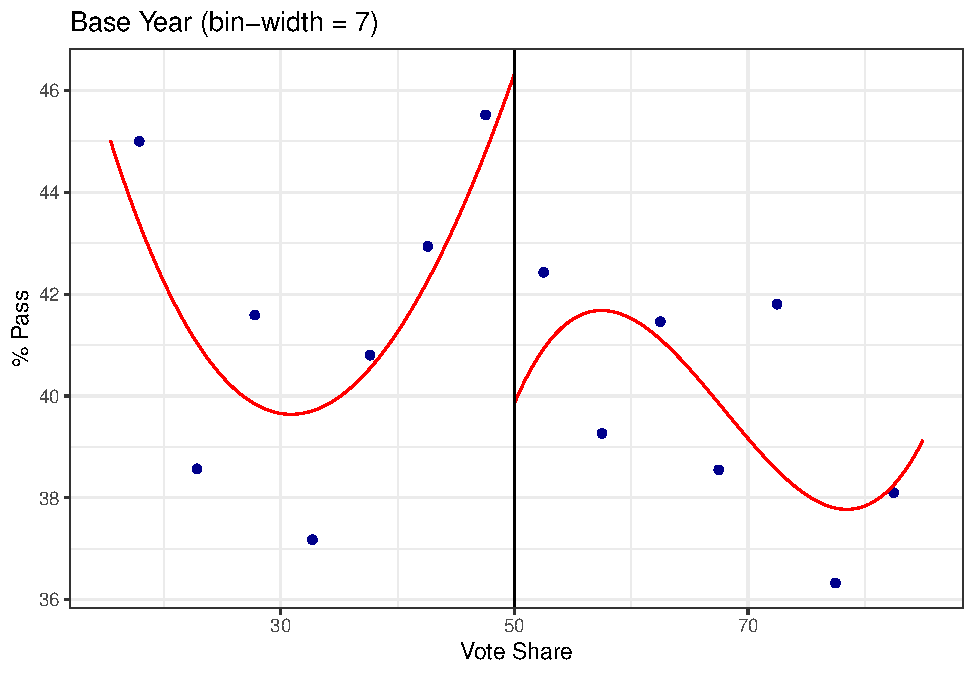
\includegraphics{Ogle_MicroMetricsAssignment_5_Q1_files/figure-latex/unnamed-chunk-2-1.pdf}

\begin{Shaded}
\begin{Highlighting}[]
\CommentTok{# Base +2 Year}
\KeywordTok{rdplot}\NormalTok{(}\DataTypeTok{y =}\NormalTok{ restrict}\OperatorTok{$}\NormalTok{passrate2, }\DataTypeTok{x =}\NormalTok{ restrict}\OperatorTok{$}\NormalTok{vote, }\DataTypeTok{c =} \DecValTok{50}\NormalTok{, }\DataTypeTok{p =} \DecValTok{3}\NormalTok{, }\DataTypeTok{nbins =} \DecValTok{7}\NormalTok{, }\DataTypeTok{title =} \StringTok{"Base + 2 Years (bin-width = 7)"}\NormalTok{, }\DataTypeTok{x.label=} \StringTok{"Vote Share"}\NormalTok{, }\DataTypeTok{y.label =} \StringTok{"% Pass"}\NormalTok{)}
\end{Highlighting}
\end{Shaded}

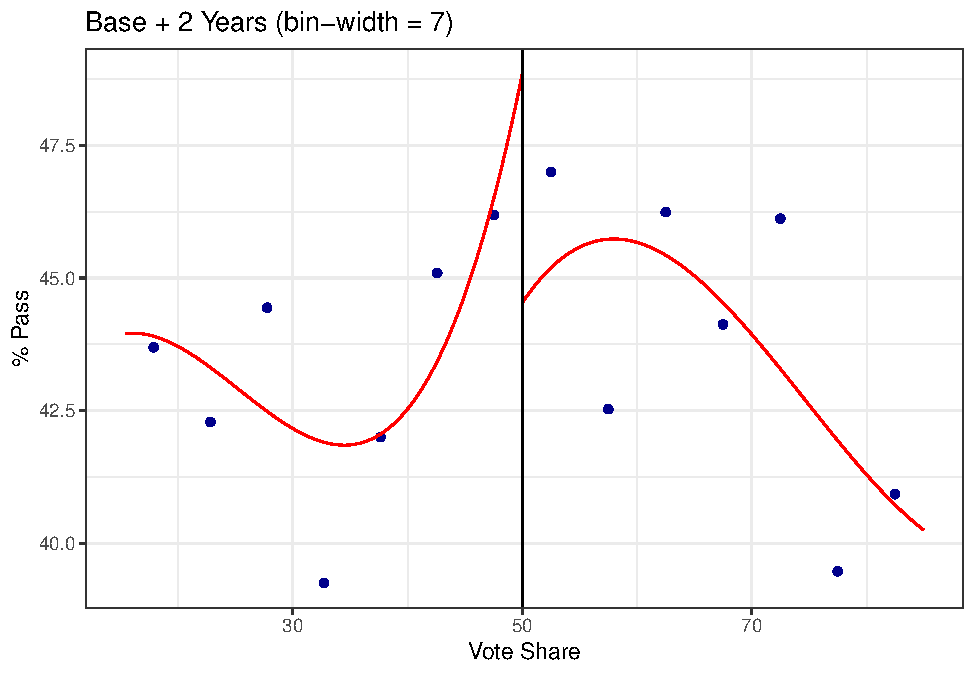
\includegraphics{Ogle_MicroMetricsAssignment_5_Q1_files/figure-latex/unnamed-chunk-2-2.pdf}

\begin{Shaded}
\begin{Highlighting}[]
\CommentTok{# % change}
\KeywordTok{rdplot}\NormalTok{(}\DataTypeTok{y =}\NormalTok{ restrict}\OperatorTok{$}\NormalTok{percentage_change, }\DataTypeTok{x =}\NormalTok{ restrict}\OperatorTok{$}\NormalTok{vote, }\DataTypeTok{p =} \DecValTok{1}\NormalTok{, }\DataTypeTok{nbins =} \DecValTok{7}\NormalTok{, }\DataTypeTok{c =} \DecValTok{50}\NormalTok{, }\DataTypeTok{title =} \StringTok{"Change (bin-width = 7)"}\NormalTok{, }\DataTypeTok{x.label=} \StringTok{"Vote Share"}\NormalTok{, }\DataTypeTok{y.label =} \StringTok{"% Pass"}\NormalTok{)}
\end{Highlighting}
\end{Shaded}

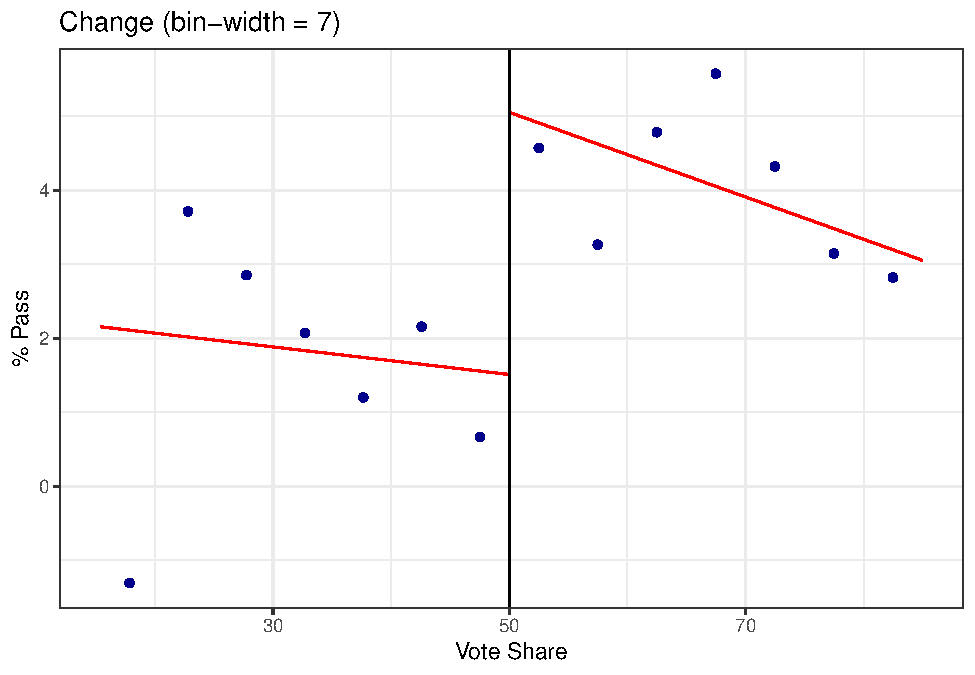
\includegraphics{Ogle_MicroMetricsAssignment_5_Q1_files/figure-latex/unnamed-chunk-2-3.pdf}

\begin{Shaded}
\begin{Highlighting}[]
\CommentTok{# Base Year}
\KeywordTok{rdplot}\NormalTok{(}\DataTypeTok{y =}\NormalTok{ restrict}\OperatorTok{$}\NormalTok{passrate0, }\DataTypeTok{x =}\NormalTok{ restrict}\OperatorTok{$}\NormalTok{vote , }\DataTypeTok{c =} \DecValTok{50}\NormalTok{, }\DataTypeTok{p =} \DecValTok{3}\NormalTok{, }\DataTypeTok{nbins =} \DecValTok{2}\NormalTok{, }\DataTypeTok{title =} \StringTok{"Base Year (bin-width = 2)"}\NormalTok{, }\DataTypeTok{x.label=} \StringTok{"Vote Share"}\NormalTok{, }\DataTypeTok{y.label =} \StringTok{"% Pass"}\NormalTok{)}
\end{Highlighting}
\end{Shaded}

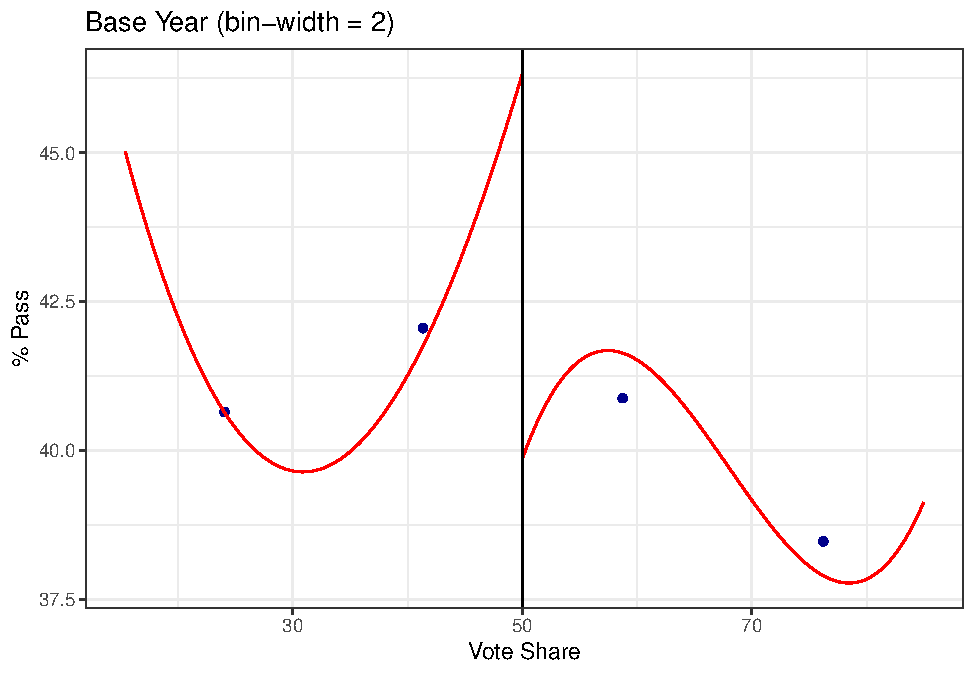
\includegraphics{Ogle_MicroMetricsAssignment_5_Q1_files/figure-latex/unnamed-chunk-2-4.pdf}

\begin{Shaded}
\begin{Highlighting}[]
\CommentTok{# Base +2 Year}
\KeywordTok{rdplot}\NormalTok{(}\DataTypeTok{y =}\NormalTok{ restrict}\OperatorTok{$}\NormalTok{passrate2, }\DataTypeTok{x =}\NormalTok{ restrict}\OperatorTok{$}\NormalTok{vote, }\DataTypeTok{c =} \DecValTok{50}\NormalTok{, }\DataTypeTok{p =} \DecValTok{3}\NormalTok{, }\DataTypeTok{nbins =} \DecValTok{2}\NormalTok{, }\DataTypeTok{title =} \StringTok{"Base + 2 Years (bin-width = 2)"}\NormalTok{, }\DataTypeTok{x.label=} \StringTok{"Vote Share"}\NormalTok{, }\DataTypeTok{y.label =} \StringTok{"% Pass"}\NormalTok{)}
\end{Highlighting}
\end{Shaded}

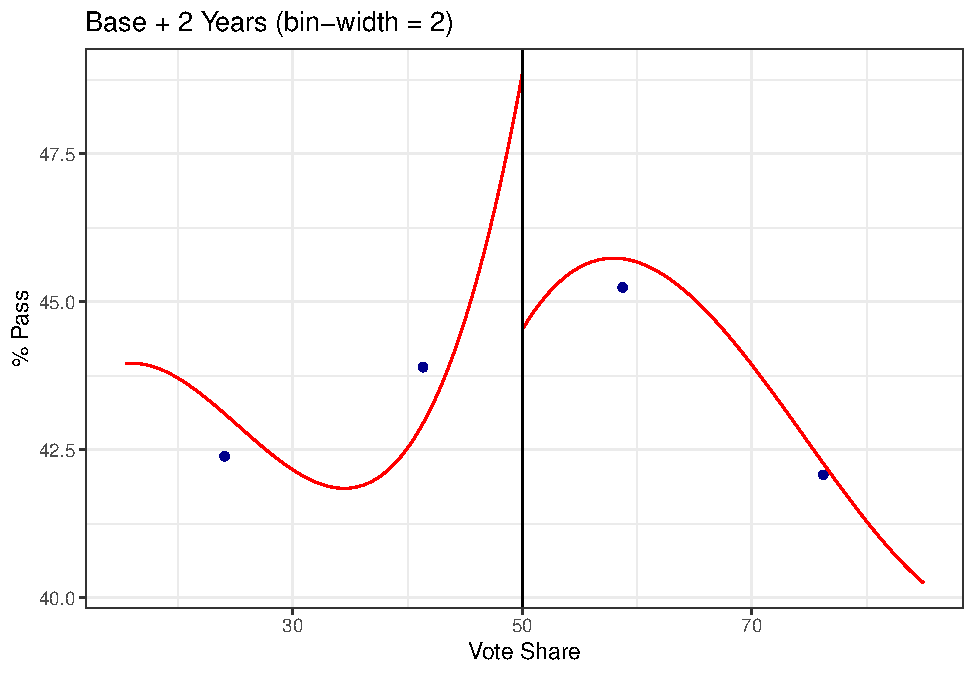
\includegraphics{Ogle_MicroMetricsAssignment_5_Q1_files/figure-latex/unnamed-chunk-2-5.pdf}

\begin{Shaded}
\begin{Highlighting}[]
\CommentTok{# % change}
\KeywordTok{rdplot}\NormalTok{(}\DataTypeTok{y =}\NormalTok{ restrict}\OperatorTok{$}\NormalTok{percentage_change, }\DataTypeTok{x =}\NormalTok{ restrict}\OperatorTok{$}\NormalTok{vote, }\DataTypeTok{p =} \DecValTok{1}\NormalTok{, }\DataTypeTok{nbins =} \DecValTok{2}\NormalTok{, }\DataTypeTok{c =} \DecValTok{50}\NormalTok{, }\DataTypeTok{title =} \StringTok{"Change (bin-width = 2)"}\NormalTok{, }\DataTypeTok{x.label=} \StringTok{"Vote Share"}\NormalTok{, }\DataTypeTok{y.label =} \StringTok{"% Pass"}\NormalTok{)}
\end{Highlighting}
\end{Shaded}

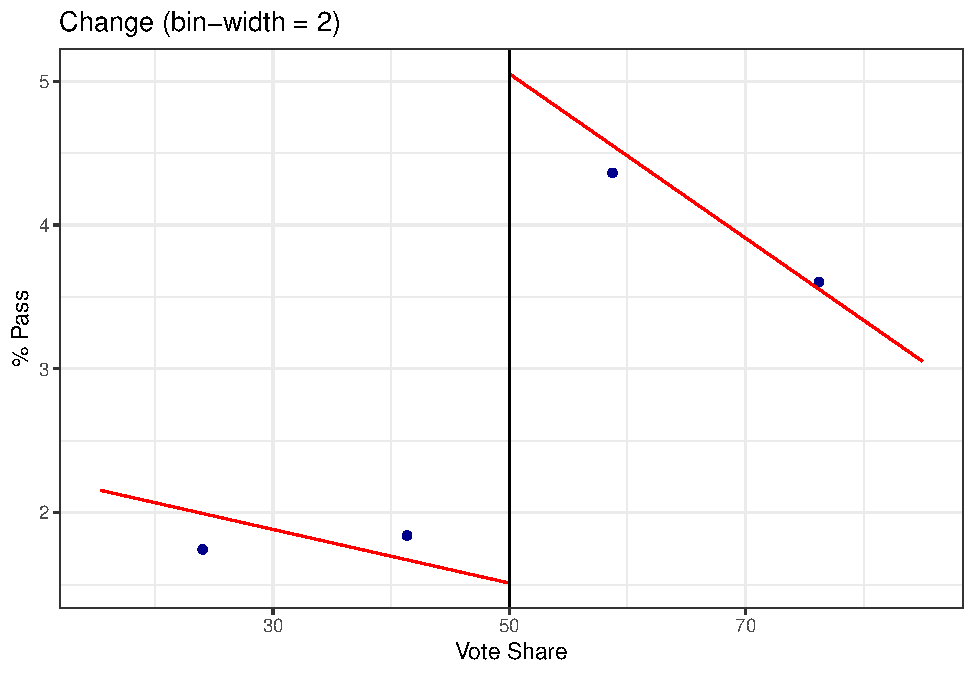
\includegraphics{Ogle_MicroMetricsAssignment_5_Q1_files/figure-latex/unnamed-chunk-2-6.pdf}

From the graphs above we can see that as you decrease the bin size from
7 which is what Clark uses in the paper for Figure 8. We can see that
there is no difference in terms of the lines of best fit, however, we
can better visualize the data with a higher bin width. We see more of
the data points.

\begin{enumerate}
\def\labelenumi{(\alph{enumi})}
\setcounter{enumi}{2}
\item
\end{enumerate}

Clark restricts his sample to those schools with votes from 15\% and
85\% because he wants to reduce bias from outliers from schools who were
very opposed or very for autonomy. For example schools with high vote
shares may have been under threat of closure, whilst few schools
received very low vote shares. Additionally, RD necessitates that in
order to estimate the average effect of a treatment you look at an
arbitrary cutoff and evaluate the treatment effects before and after the
cutoff. Additionally they saw that schools outside this interval have
different baseline characteristics and are less likely to survive. Clark
needs to estimate around the cutoff, 50, which is inside the (15,85)
interval. Other columns have functions of vote share because vote share
is the forcing variable in this Fuzzy Regression Discontinuity model.
Fuzzy RD exploits discontinuities in the probability of treatment
conditional on a variate. The discontinuity, here is Vote share, and it
becomes the IV for the treatment status. Which is why Table 3a includes
functions of vote share both on their own and interacted with the
win/lose variable.

\begin{enumerate}
\def\labelenumi{(\alph{enumi})}
\setcounter{enumi}{3}
\item
\end{enumerate}

\begin{Shaded}
\begin{Highlighting}[]
\NormalTok{restrict}\OperatorTok{$}\NormalTok{vote_share <-}\StringTok{ }\NormalTok{restrict}\OperatorTok{$}\NormalTok{vote}\OperatorTok{/}\DecValTok{100}

\CommentTok{# model_d_1 <- rdrobust(restrict$vote_share, restrict$win, c = 0.5, all=T)}

\CommentTok{# stargazer(model_d_1, column.labels=c("Non-Grammar Schools with Vote Shares in [15,85] interval"), title="Regression Results (d)", align=TRUE, notes = "Standard errors in parentheses", notes.align = "l")}
\end{Highlighting}
\end{Shaded}

\begin{table}[!htbp] \centering 
  \caption{Regression Results (d)} 
  \label{} 
\begin{tabular}{@{\extracolsep{5pt}}lD{.}{.}{-3} } 
\\[-1.8ex]\hline 
\hline \\[-1.8ex] 
 & \multicolumn{1}{c}{\textit{Dependent variable:}} \\ 
\cline{2-2} 
 & \multicolumn{1}{c}{Non-Grammar Schools with Vote Shares in [15,85] interval} \\ 
\hline \\[-1.8ex] 
 Win & -0.000^{***} \\ 
  & (0.000) \\ 
  & \\ 
 lose &  \\ 
  &  \\ 
  & \\ 
 percentage\_change & 0.000 \\ 
  & (0.000) \\ 
  & \\ 
 vote:lose & 1.000^{***} \\ 
  & (0.000) \\ 
  & \\ 
 vote:win & 1.000^{***} \\ 
  & (0.000) \\ 
  & \\ 
 Constant & -0.000^{***} \\ 
  & (0.000) \\ 
  & \\ 
\hline \\[-1.8ex] 
Observations & \multicolumn{1}{c}{524} \\ 
R$^{2}$ & \multicolumn{1}{c}{1.000} \\ 
Adjusted R$^{2}$ & \multicolumn{1}{c}{1.000} \\ 
Residual Std. Error & \multicolumn{1}{c}{0.000 (df = 519)} \\ 
F Statistic & \multicolumn{1}{c}{34,064,124,303,065,597,294,021,672,173,568.000$^{***}$ (df = 4; 519)} \\ 
\hline 
\hline \\[-1.8ex] 
\textit{Note:}  & \multicolumn{1}{l}{$^{*}$p$<$0.1; $^{**}$p$<$0.05; $^{***}$p$<$0.01} \\ 
 & \multicolumn{1}{l}{Standard errors in parentheses} \\ 
\end{tabular} 
\end{table}

\begin{enumerate}
\def\labelenumi{(\alph{enumi})}
\setcounter{enumi}{4}
\item
\item
\item
\item
\item
\item
\end{enumerate}

\end{document}
